\documentclass[12pt]{report}
\title{Capstone Project - RR4-IP \\Unmanned Recon and Surveillance Aircraft (U.R.S.A.) \\ \Huge Final Report}
\author{\large Lachlan Dowling - 682434 \\ Isaac Hook - 720679 \\ Hao Tang - 640207 }
\date{2017}
\setlength\parindent{0pt}
\usepackage[margin=0.8in]{geometry}
\usepackage{amssymb,amsmath}
\usepackage{xr}
\usepackage{booktabs}
\usepackage{multirow}
\usepackage{array}
\renewcommand{\arraystretch}{1.5}
\usepackage{bm}
\usepackage{graphicx}
\usepackage[]{algorithm2e}
\usepackage{pgfplots}
\usepackage{afterpage}
\pgfplotsset{compat=1.12}
\usepackage{soul}
\usepackage{pdfpages}
\usepackage{xstring}
\usepackage{siunitx}
\usepackage{tikz}
\usepackage{caption}
\usepackage{subcaption}
\usepackage{float}
\usepackage{fancyhdr}
\usepackage{mathtools}
\usepackage{titlesec}
\usepackage{hyperref}
\usepackage{listings}
\usepackage{rotating}
\usepackage{pdflscape}
\usepackage{appendix}
\usepackage{subfiles}
\usepackage{setspace}
\usepackage[americancurrents, americanvoltages,siunitx]{circuitikz}
\newcolumntype{P}[1]{>{\centering\arraybackslash}p{#1}}
\pagestyle{fancy}
\fancyhf{}
\lhead{Capstone Project}
\rhead{Final Report: RR4-IP}
\rfoot{Page \thepage}
\DeclareSIUnit\dBm{dBm}
\newcommand*\circled[1]{\tikz[baseline=(char.base)]{\node[shape=circle,draw,inner sep=2pt] (char) {#1};}}
\let\oldhat\hat
\renewcommand{\hat}[1]{\oldhat{\bm{#1}}}
\lstset{basicstyle=\ttfamily,
    showstringspaces=false,
    keywordstyle=\color{blue},
    stringstyle=\color{red}\ttfamily,
    commentstyle=\color{green}\ttfamily
}
\renewcommand\thesection{\arabic{chapter}.\arabic{section}.}
\renewcommand\thesubsection{\arabic{chapter}.\arabic{section}.\arabic{subsection}. \ }
\renewcommand\thesubsubsection{}
\renewcommand\theparagraph{(\roman{paragraph})}
\renewcommand\thesubfigure{\roman{subfigure}}

\titleformat{\section}[frame]
{\normalfont}
{\filright
\footnotesize}
{8pt}
{\Large\bfseries\filcenter \enspace \thesection \enspace}

\titleformat{\subsection}[hang]
{\normalfont\sffamily}
{\large\bfseries\thesubsection}{1.5em}{\large\bfseries}


\titleformat{\subsubsection}[hang]
{\normalfont\sffamily}
{\bfseries{\thesubsubsection}}{.5em}{\bfseries}

\setcounter{secnumdepth}{4}
\titleformat{\paragraph}[runin]
{\normalfont\sffamily}
{\theparagraph}{.5em}{}

\everymath={\displaystyle}

\newenvironment{changemargin}[2]{%
\begin{list}{}{%
\setlength{\topsep}{0pt}%
\setlength{\leftmargin}{#1}%
\setlength{\rightmargin}{#2}%
\setlength{\listparindent}{\parindent}%
\setlength{\itemindent}{\parindent}%
\setlength{\parsep}{\parskip}%
}%
\item[]}{\end{list}}
\onehalfspacing

\begin{document}
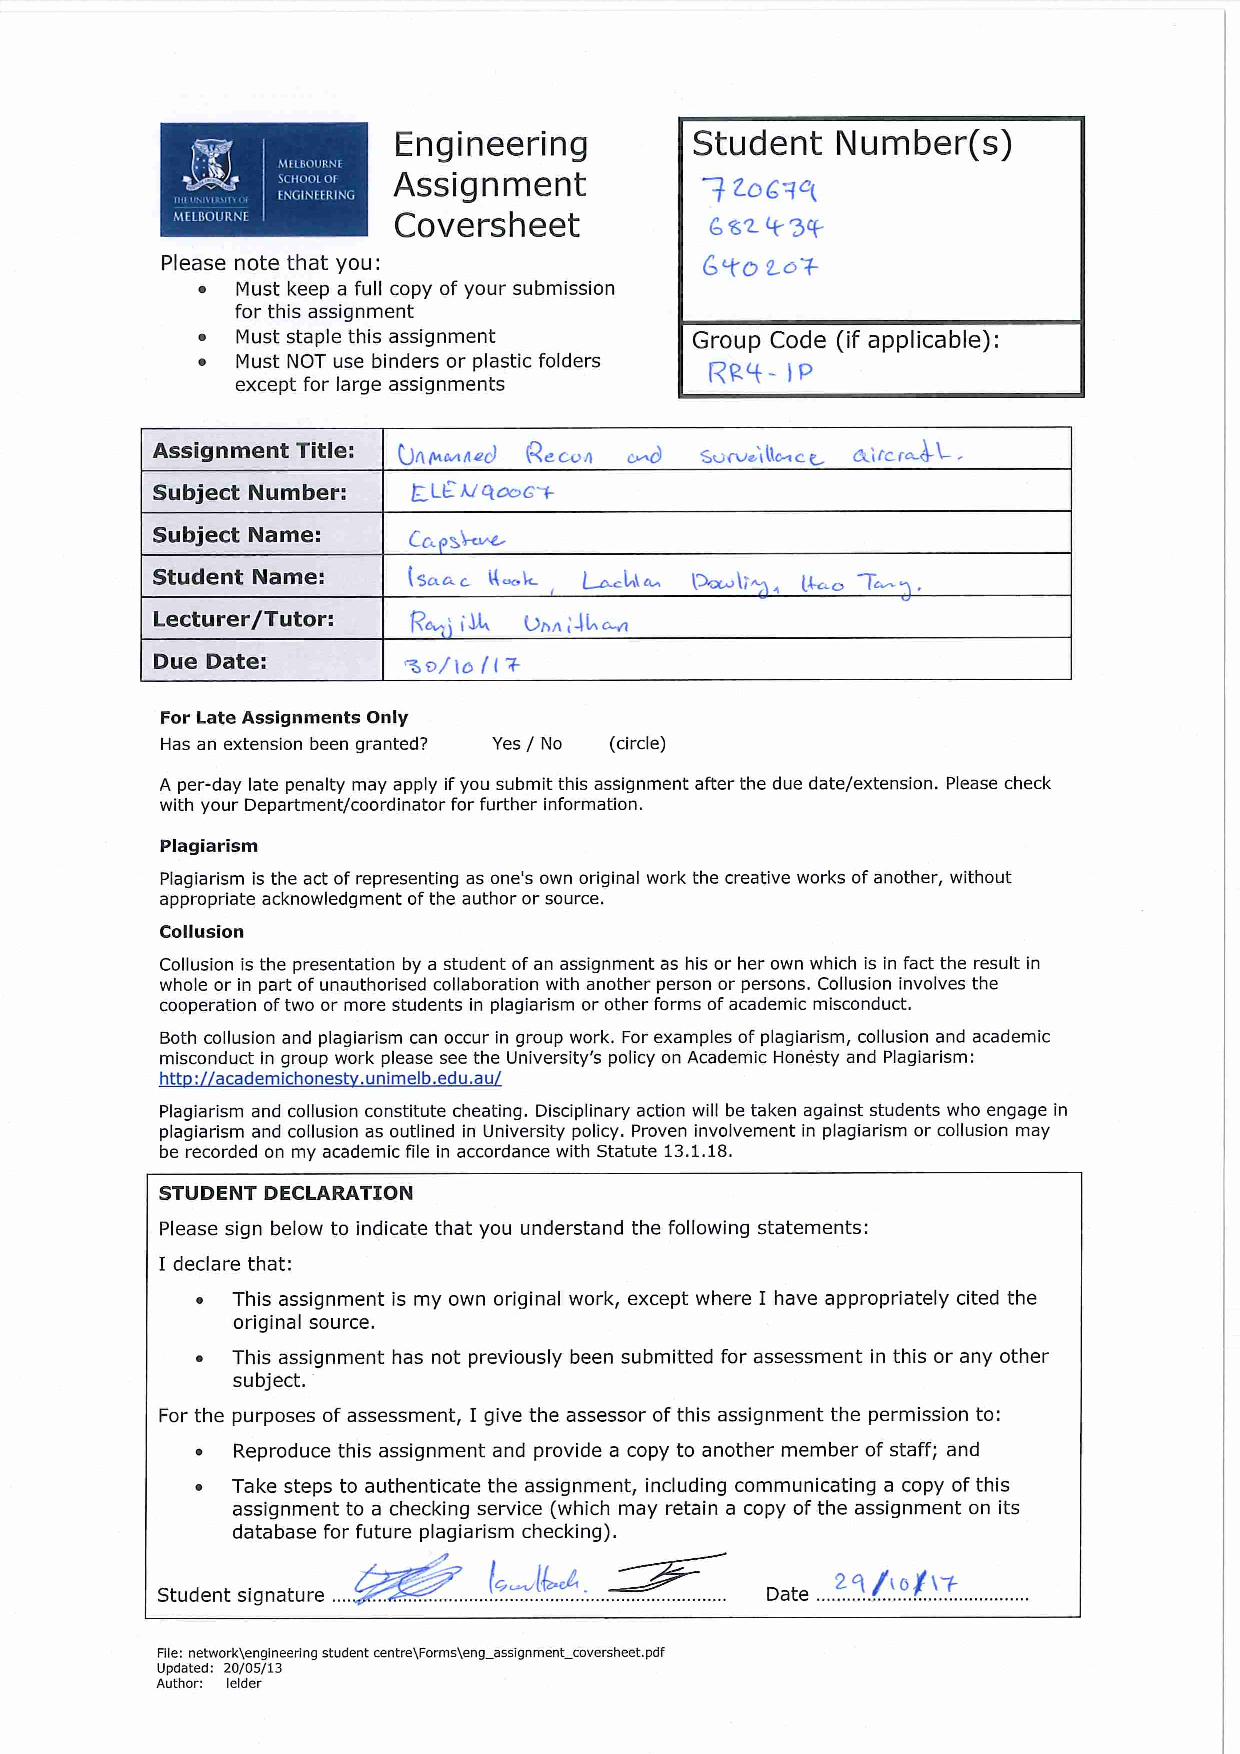
\includepdf[pages=-]{coversheet.pdf}
\thispagestyle{empty}
    \maketitle
    \thispagestyle{empty}
    
    \newpage

    \clearpage
    \setcounter{page}{1}

\subfile{abstract.tex}
\tableofcontents


\subfile{introduction.tex}
\subfile{litreview.tex}
\subfile{designdevelopment.tex}
\subfile{implementation.tex}
\subfile{results.tex}
\subfile{conclusion.tex}

\bibliography{capstone_bib}{}
\bibliographystyle{IEEEtran}

\appendix
\appendixpage
Appendices have been provided in a USB drive along with this report. Alternatively, the appendices can be accessed at \url{https://drive.google.com/open?id=0B64fzCinYuhLNW1KeU1kM1B5c0E}. Table \ref{tab:apptable} provides a summary of appendices. Full code developed for PX4 and ROS has not been provided in the appendices due to size constraints but can be accessed at \url{https://github.com/ursa-drone/}.

\begin{table}[H]
\centering
    \begin{tabular}{|c|c|}
        \hline
        Appendix & Description\\
        \hline
        A & BOM \\
        B & BCM2835 ARM Peripherals datasheet\\
        C & HC-SR04 datasheet\\
        D & PCA9685 datasheet\\
        E & MS5611 datasheet\\
        F & MPU9250 datasheet\\
        G & ADS1115 datasheet\\
        H & MATLAB code written to tune cost functions\\
        I & Example of URSA team contributing to further PX4 development\\
        J & Video of flight tests undertaken\\
        \hline
    \end{tabular}
\caption{Summary of appendices \label{tab:apptable}}
\end{table}


\end{document}